%% Преамбула TeX-файла

% 1. Стиль и язык
\documentclass{G7-32} % Стиль (по умолчанию размер шрифта 14pt)

% Остальные стандартные настройки убраны в preamble.inc.tex.
\include{preamble.inc}

% Настройки листингов.
\ifPDFTeX
\include{listings.inc}
\else
\usepackage{local-minted}
\fi

% Полезные макросы листингов.
\include{macros.inc}

% Стиль титульного листа и заголовки
%\include{00-title}


\begin{document}

\frontmatter % выключает нумерацию ВСЕГО; здесь начинаются ненумерованные главы: реферат, введение, глоссарий, сокращения и прочее.

% Титульная страница
%\maketitle %создает титульную страницу\\
%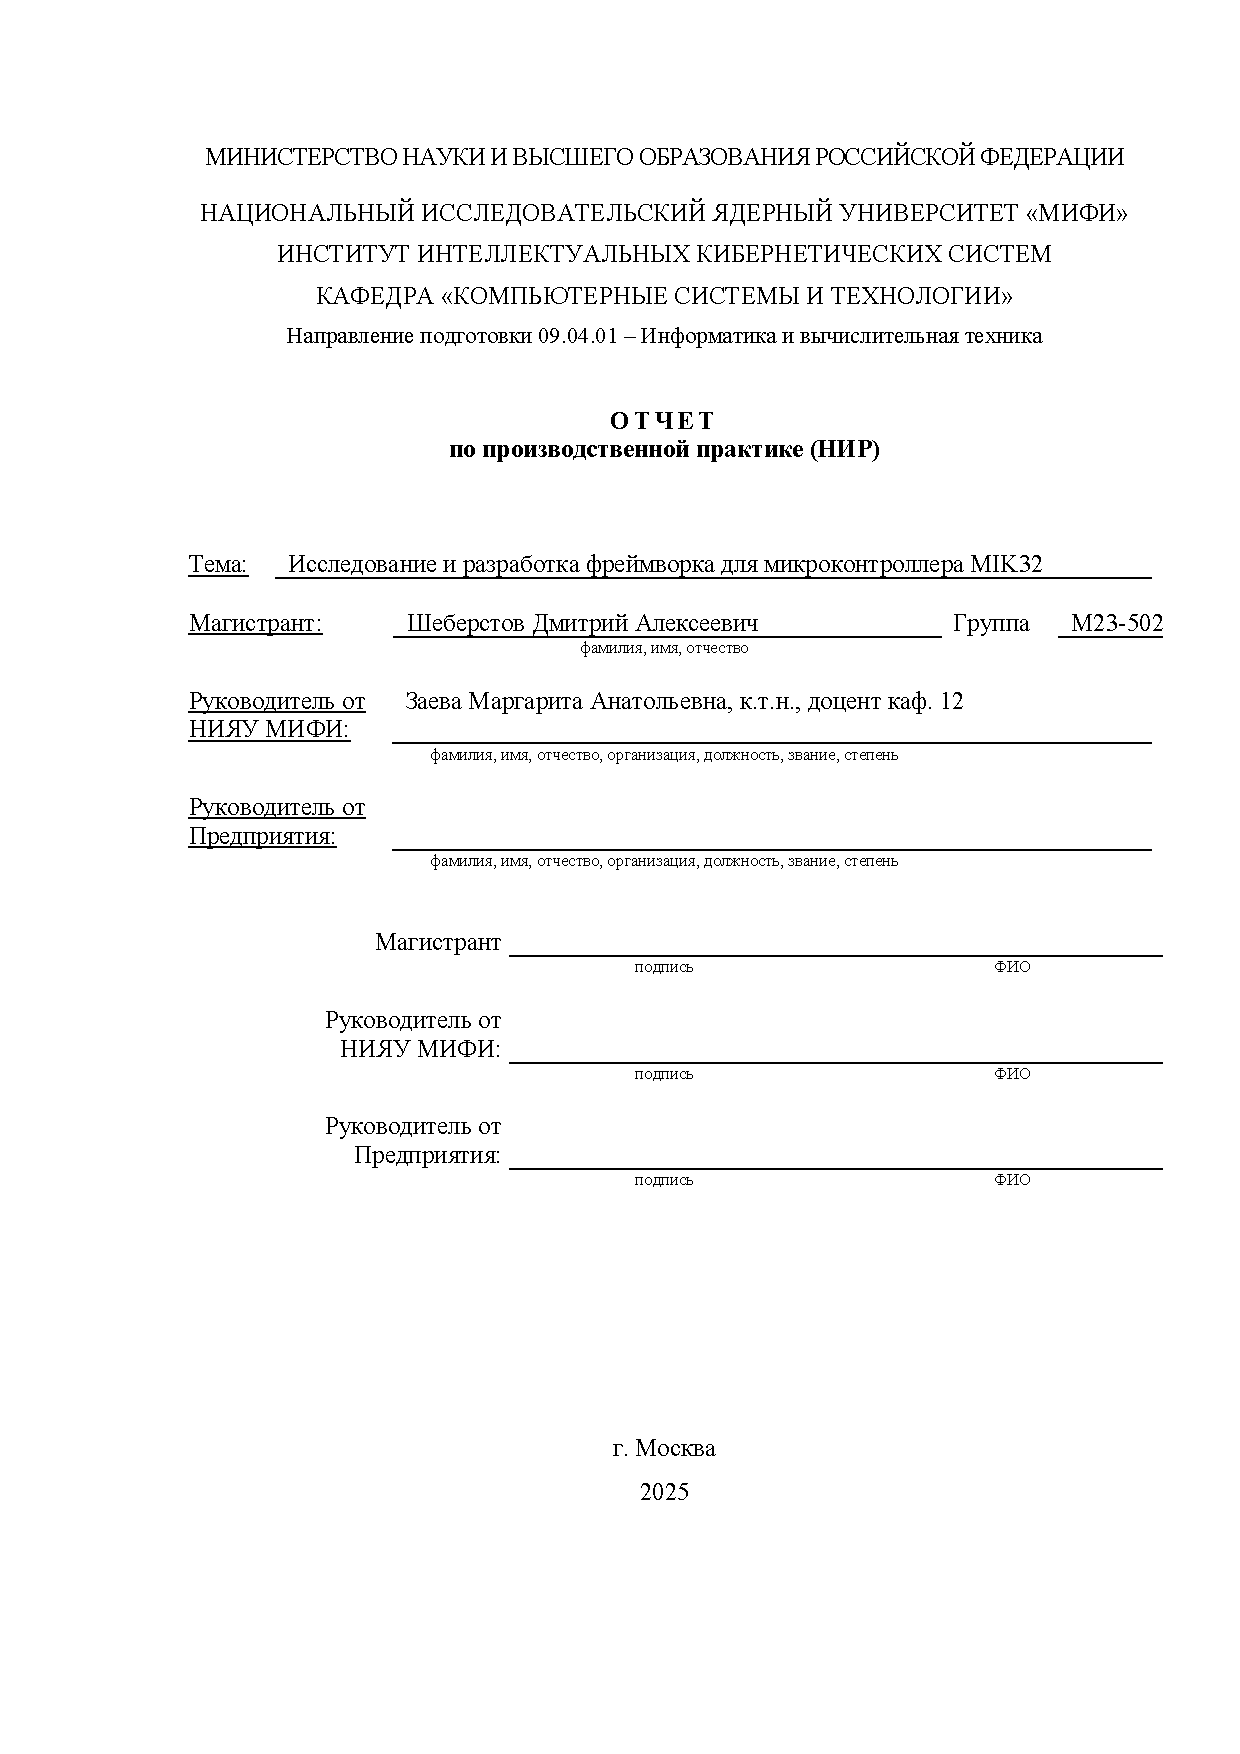
\includepdf[pages=-]{titlepage1.pdf}

\includepdf[pages=-]{titlepage.pdf}

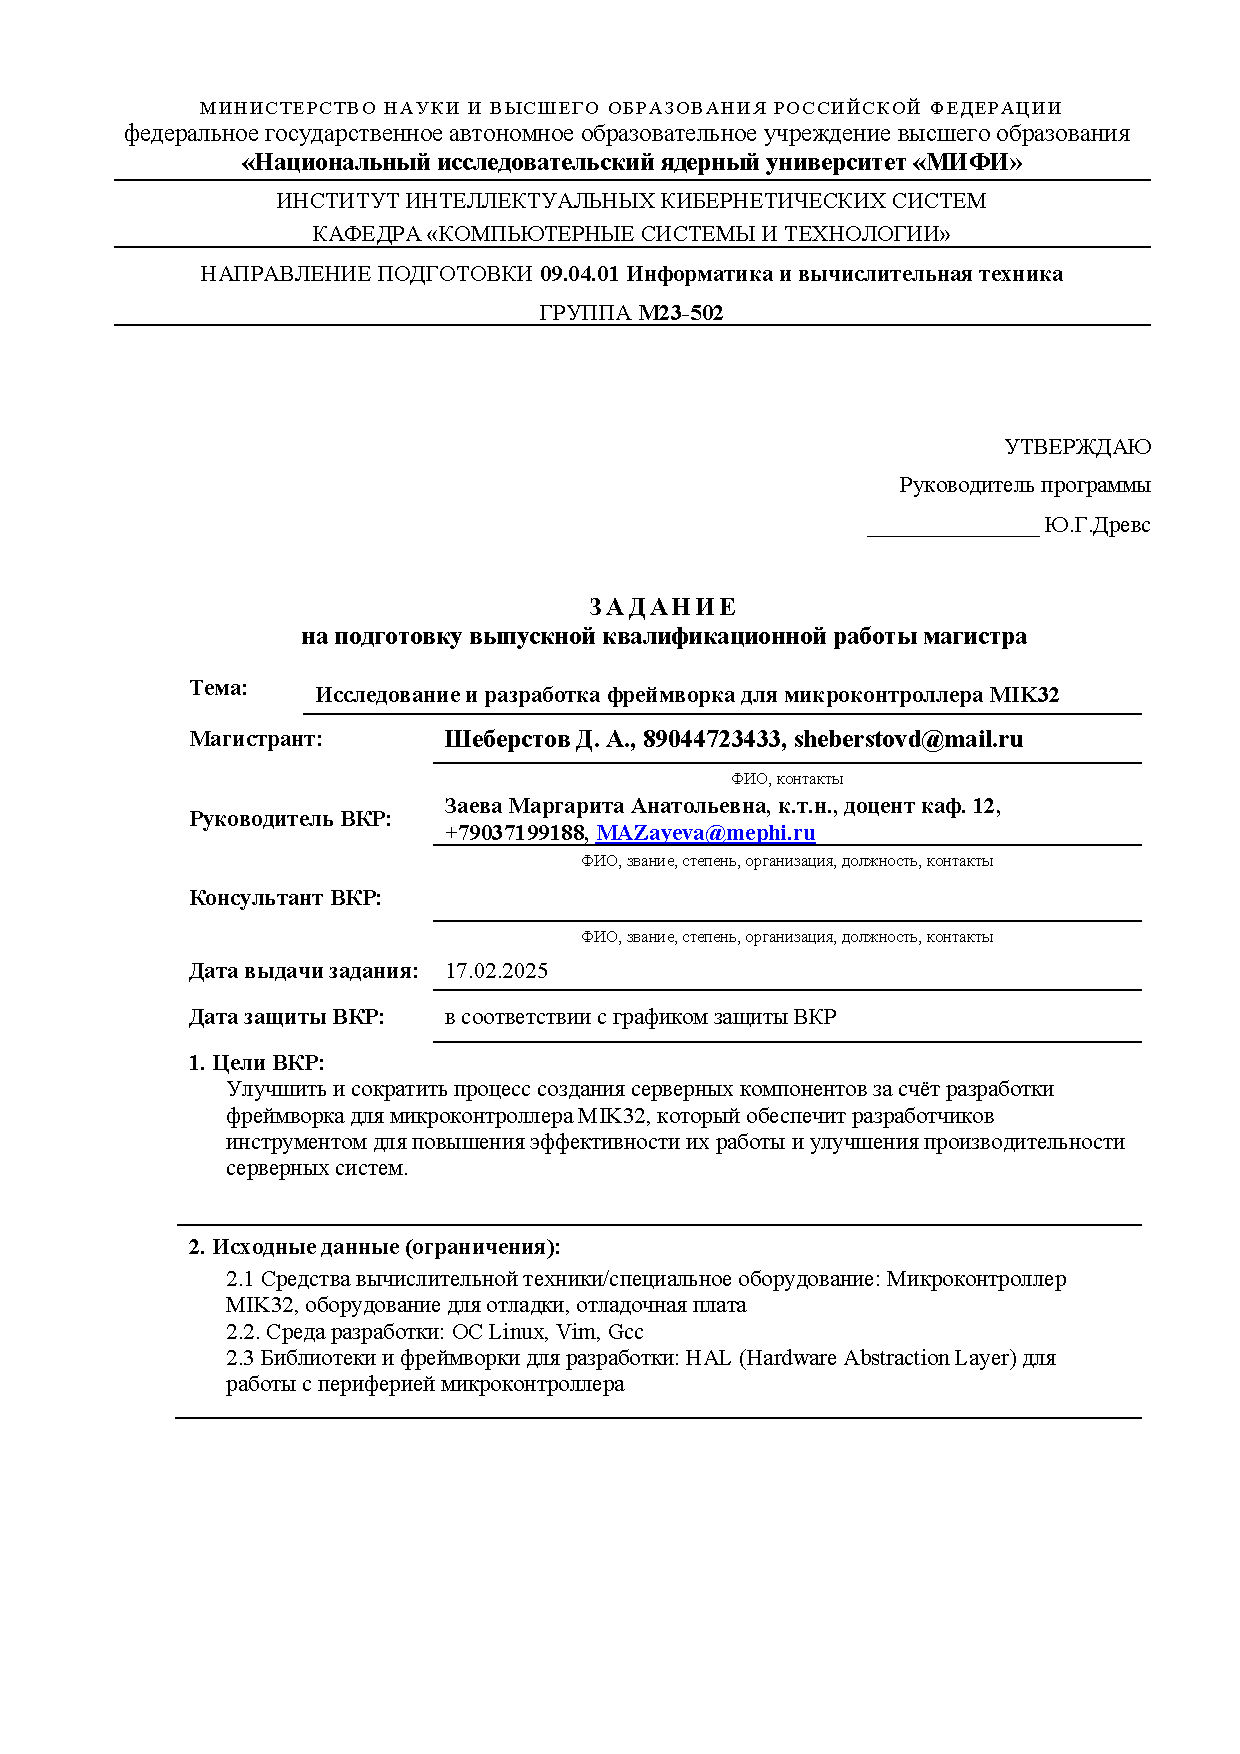
\includepdf[pages=-]{task.pdf}

%\begin{executors}
%\personalSignature{Первый исполнитель}{ФИО}
%
%\personalSignature{Второй исполнитель}{ФИО}
%\end{executors}


%\listoffigures                         % Список рисунков

%\listoftables                          % Список таблиц

%\NormRefs % Нормативные ссылки 
% Команды \breakingbeforechapters и \nonbreakingbeforechapters
% управляют разрывом страницы перед главами.
% По-умолчанию страница разрывается.

% \nobreakingbeforechapters
% \breakingbeforechapters

% Также можно использовать \Referat, как в оригинале
\begin{abstract}
\begin{center}
\textbf{к выпускной квалификационной работе магитсра на тему «Исследование и разработка фреймворка для микроконтроллера MIK32»}

\textbf{Шеберстова Дмитрия Алексеевича}

\textbf{Руководитель - Заева Маргарита Анатольевна, к.т.н., НИЯУ МИФИ, ИИКС, доцент}

\end{center}

    Пояснительная записка к выпускной квалификационной работе магистра (диссертации) \pageref{LastPage}\,стр.%
    \ifnum \totfig >0
    , \totfig~рис.%
    \fi
    \ifnum \tottab >0
    , \tottab~табл.%
    \fi
    %
    \ifnum \totbib >0
    , \totbib~источн.%
    \fi
    %
    \ifnum \totapp >0
    , \totapp~прил.%
    \else
    .%
    \fi

ВСТРОЕННЫЕ СИСТЕМЫ, ИМПОРТОЗАМЕЩЕНИЕ, МИКРОКОНТРОЛЛЕР, ОТЕЧЕСТВЕННЫЕ ТЕХНОЛОГИИ, ФРЕЙМВОРК, I2C, GPIO, HAL, RISC-V

Актуальность исследования обусловлена необходимостью создания отечественных решений в области микроэлектроники и разработки инструментов программирования для российских микроконтроллеров. Микроконтроллер MIK32, построенный на открытой архитектуре RISC-V, представляет собой платформу для импортозамещения в критически важных отраслях.

Объектом исследования является микроконтроллер MIK32. Предметом исследования выступают методы и средства разработки программного обеспечения для данного микроконтроллера, включая архитектурные решения фреймворков и подсистемы управления периферийными устройствами.

Цель работы заключается в упрощении процесса разработки встроенных приложений за счет создания прототипа фреймворка для микроконтроллера MIK32, который обеспечит абстракцию аппаратных ресурсов.

Для достижения поставленной цели решались задачи: анализ архитектурных особенностей микроконтроллера MIK32 и существующих решений для RISC-V платформ; проектирование многоуровневой архитектуры фреймворка с четким разделением аппаратно-зависимых и аппаратно-независимых компонентов; разработка унифицированных подсистем управления GPIO и I2C; реализация драйверов для внешних расширителей портов; практическая апробация фреймворка в промышленных проектах.

Методы исследования включают: анализ архитектуры микроконтроллеров и существующих фреймворков; проектирование с применением паттернов абстракции; экспериментальное тестирование на реальных аппаратных платформах.

Научная новизна заключается в разработке архитектуры фреймворка, адаптированной к особенностям отечественного микроконтроллера MIK32, обеспечивающую совместимость с широким спектром периферийных устройств.

Практическая значимость подтверждается успешным применением фреймворка в двух промышленных проектах: системе управления нагревом Heating Unit и системе управления вентиляторами Midplane. Разработанный фреймворк способствует ускорению разработки встроенных систем на базе MIK32 и повышению конкурентоспособности отечественных технологий.

\end{abstract}

%%% Local Variables: 
%%% mode: latex
%%% TeX-master: "rpz"
%%% End: 


\tableofcontents

\printnomenclature % Автоматический список сокращений

\Introduction

Современное состояние мировой микроэлектроники характеризуется интенсивным развитием архитектур микроконтроллеров и растущими требованиями к разработки встроенных систем. В условиях геополитической нестабильности и технологических ограничений особую актуальность приобретает создание отечественных решений в области микроэлектроники, способных обеспечить технологическую независимость критически важных отраслей экономики.

Микроконтроллер MIK32 демонстрирует потенциал отечественных технологий в создании конкурентоспособных решений. Однако использование потенциала данного микроконтроллера требует создания специализированного программного обеспечения, которое обеспечит удобство разработки и оптимальное использование аппаратных ресурсов.

Актуальность исследования обусловлена несколькими факторами. Во-первых, растущая потребность в импортозамещении микроэлектронных компонентов требует не только создания отечественной элементной базы, но и разработки соответствующего программного инструментария. Во-вторых, открытая архитектура RISC-V предоставляет уникальные возможности для создания оптимизированных решений без ограничений проприетарных лицензий. В-третьих, отсутствие зрелых инструментов разработки для MIK32 создает барьеры для широкого внедрения данного микроконтроллера в промышленных применениях.

Анализ современного состояния разработки встроенных систем показывает, что фреймворки играют важную роль в повышении производительности разработчиков и качества создаваемых решений. Существующие фреймворки и операционные системы реального времени для микроконтроллеров, такие как STM32CubeHAL для семейства STM32, Mbed OS, FreeRTOS, Zephyr или ESP-IDF для ESP32, демонстрируют преимущества в скорости разработки и надежности результирующих систем. Однако специфика архитектуры MIK32 и требования отечественного рынка обусловливают необходимость создания специализированного решения.

Объектом исследования является микроконтроллер MIK32 (К1948ВК018) как представитель класса 32-битных микроконтроллеров с архитектурой RISC-V, включая его аппаратную архитектуру и периферийные устройства.

Предметом исследования выступают методы и принципы проектирования программных фреймворков для микроконтроллеров, включая архитектурные паттерны абстракции аппаратных ресурсов, подходы к созданию универсальных программных интерфейсов и механизмы обеспечения переносимости программного кода.

Цель работы заключается в упрощении процесса разработки встроенных приложений за счет исследовании и создания прототипа фреймворка для микроконтроллера MIK32, который обеспечит абстракцию аппаратных ресурсов.

Для достижения поставленной цели определены следующие задачи:

\begin{enumerate}
	\item Выполнить сравнительный анализ существующих фреймворков и операционных систем реального времени для микроконтроллеров с целью выявления лучших практик и архитектурных решений.
	\item Провести анализ особенностей микроконтроллера MIK32, включая изучение процессорного ядра SCR1, периферийных устройств и специфики программной модели RISC-V.
	\item Разработать прототип многоуровневого фреймворка, обеспечивающую разделение между аппаратно-зависимыми и аппаратно-независимыми компонентами.
	\item Спроектировать и реализовать унифицированные подсистемы управления периферийными устройствами.
	\item Провести апробацию фреймворка в реальных промышленных проектах различной сложности.
\end{enumerate}

Методы исследования включают: анализ архитектуры микроконтроллеров и существующих программных решений; экспериментальное моделирование и тестирование на реальных аппаратных платформах; сравнительный анализ с существующими решениями.

Научная новизна работы заключается в разработке модульной архитектуры фреймворка, которая учитывает требования российского рынка встренных стистем.
Практическая значимость исследования определяется успешной апробацией фреймворка в промышленных проектах различной сложности, подтвердившей его универсальность и практическую применимость. Формированием методологической базы для создания аналогичных фреймворков для других отечественных микроконтроллеров. Созданием готового к использованию инструментария для разработки встроенных систем на базе MIK32, что способствует ускорению процесса внедрения отечественного микроконтроллера в промышленные применения.

\Abbrev{API}{Application Programming Interface — интерфейс прикладного программирования}
\Abbrev{HAL}{Hardware Abstraction Layer — слой абстракции аппаратного обеспечения}
\Abbrev{GPIO}{General Purpose Input/Output — порты ввода-вывода общего назначения}
\Abbrev{I2C}{Inter-Integrated Circuit — двухпроводной последовательный интерфейс}
\Define{Фреймворк}{программная платформа, определяющая структуру программной системы и облегчающая разработку приложений}


\mainmatter % это включает нумерацию глав и секций в документе ниже


\chapter{Обзор существующих решений по разработке фреймворков для микроконтроллеров}

\label{cha:theory}

Разработка программного обеспечения для микроконтроллеров требует учёта специфики аппаратных ограничений, включая объёмы памяти, энергоэффективность и поддержку периферийных устройств\cite{Harris2021}. Данная глава посвящена теоретическому анализу базовых концепций, принципов и технологий, лежащих в основе разработки фреймворков для микроконтроллеров.
\section{Микроконтроллеры в современных встраиваемых системах}

Микроконтроллеры представляют собой ключевой компонент современных встраиваемых систем, обеспечивая интеллектуальное управление различными устройствами от бытовой техники до промышленных систем управления\cite{Kernighan2019}. Первый коммерчески доступный микроконтроллер TMS1000 объединил в себе 4-битный ЦПУ, 1 КБ ПЗУ, 256-битную ОЗУ и линии ввода/вывода на одном чипе. Сегодня высокопроизводительный 32-битный микроконтроллер с 2 МБ встроенной SRAM может достигать скорости 1 ГГц, работая как минимум в 2500 раз быстрее. Современные микроконтроллеры часто классифицируют по разрядности обрабатываемых данных: 8-разрядные, 16-разрядные и 32-разрядные.

В зависимости от функционального назначения микроконтроллеры могут быть разделены на следующие основные типы:

\begin{itemize}
	\item Встраиваемые 8-разрядные микроконтроллеры
	\item 16- и 32-разрядные микроконтроллеры
	\item Цифровые сигнальные процессоры (DSP)
\end{itemize}

Существуют две основные архитектуры микроконтроллеров: архитектура фон Неймана и гарвардская архитектура\cite{MartinArch2024}. Гарвардская архитектура, характеризующаяся разделением каналов для инструкций и данных, обеспечивает более высокую производительность за счет одновременного доступа к командам и данным (\ref{fig:arch_comp}).

\begin{figure}
	\centering
	
\includegraphics[width=0.7\textwidth]{inc/img/arch-comp}
	\caption{Сравнение архитектур}
	\label{fig:arch_comp}
\end{figure}

В гарвардской архитектуре характеристики устройств памяти для инструкций и данных могут различаться. В частности, ширина слова, тактирование, технология реализации и структура адресов памяти не обязательно должны быть одинаковыми. Это позволяет оптимизировать каждый канал под конкретные требования, что особенно важно для встраиваемых систем с ограниченными ресурсами.

Современные микроконтроллеры часто используют гибридные архитектуры, сочетающие преимущества обоих подходов. Например, многие CISC-процессоры имеют раздельную кэш-память первого уровня для команд и данных, что позволяет им получать одновременно и команду, и данные для её выполнения.

Встраиваемые микроконтроллеры содержат значительное число вспомогательных устройств, что позволяет использовать минимальное количество дополнительных компонентов при интеграции в систему. Типичная структура микроконтроллера представлена на рисунке \ref{fig:mik_struct}.

\begin{figure}
	\centering
	
\includegraphics[width=0.7\textwidth]{inc/img/mik-struct}
	\caption{Структурная схема микроконтроллера}
	\label{fig:mik_struct}
\end{figure}

В состав современного микроконтроллера обычно входят следующие компоненты:

\begin{itemize}
	\item Центральный процессор (CPU)
	\item Память программ (Flash, ROM, EPROM)
	\item Память данных (RAM)
	\item Схема начального запуска (Reset)
	\item Генератор тактовых импульсов
	\item Периферийные устройства (таймеры, АЦП, ЦАП, интерфейсы связи)
\end{itemize}

\section{Архитектура RISC-V и её применение в микроконтроллерах}

RISC-V представляет собой открытую стандартную архитектуру набора инструкций, основанную на принципах RISC\cite{RISC2024}. В отличие от проприетарных архитектур, таких как ARM, AVR или x86, RISC-V является открытым стандартом, что позволяет любому производителю реализовывать его спецификации без лицензионных отчислений.

\Abbrev{RISC}{reduced instruction set computer ""--- архитектурный подход к проектированию процессоров, в которой быстродействие увеличивается за счёт такого кодирования инструкций, чтобы их декодирование было более простым, а время выполнения -- меньшим.}

RISC-V был разработан в Калифорнийском университете в Беркли, начиная с 2010 года, как перспективная архитектура, не обремененная требованиями обратной совместимости\cite{RISC2024}. Она была спроектирована не только для академических целей, но и для практического применения в реальных устройствах.

Преимущества архитектуры RISC-V для применения в микроконтроллерах:

\begin{itemize}
	\item Модульность: RISC-V состоит из базового набора инструкций (RV32I, RV64I) и опциональных расширений (M, A, F, D, C и др.), что позволяет адаптировать процессор под конкретные задачи\cite{RISC2024}.
	\item Открытость: Спецификации RISC-V доступны бесплатно под лицензией BSD, что способствует инновациям и снижает барьеры для входа новых производителей.
	\item Масштабируемость: RISC-V поддерживает 32-, 64- и 128-битные варианты адресного пространства, что обеспечивает гибкость при реализации различных классов устройств.
	\item Компактность: Расширение "C" позволяет использовать 16-битные инструкции, сокращая размер кода до 25-30\% по сравнению с базовым набором.
	\item Архитектура load-store: Инструкции RISC-V адресуют только регистры, а для взаимодействия с памятью используются специальные инструкции загрузки и сохранения.
\end{itemize}

RISC-V предлагает гибкую систему расширений набора инструкций, что позволяет создавать процессоры с различными характеристиками. Основные наборы инструкций включают:

\begin{itemize}
	\item RV32I - базовый 32-битный набор целочисленных инструкций
	\item RV64I - базовый 64-битный набор целочисленных инструкций
	\item RV32E - набор с уменьшенным количеством регистров для встраиваемых систем
\end{itemize}

Стандартные расширения включают:

\begin{itemize}
	\item I (Base Integer Instruction Set): Базовый набор целочисленных инструкций, обязательный для всех реализаций RISC-V.
	\item M (Standard Extension for Integer Multiplication and Division): Стандартное расширение для операций умножения и деления целых чисел.
	\item A (Standard Extension for Atomic Instructions): Стандартное расширение для атомарных операций, необходимых для синхронизации в многопоточных приложениях.
	\item F (Standard Extension for Single-Precision Floating-Point): Стандартное расширение для операций с плавающей точкой одинарной точности (32 бита).
	\item D (Standard Extension for Double-Precision Floating-Point): Стандартное расширение для операций с плавающей точкой двойной точности (64 бита).
	\item C (Standard Extension for Compressed Instructions): Стандартное расширение для 16-битных сжатых инструкций, позволяющее уменьшить размер кода и повысить плотность инструкций.
	\item V (Vector Extension): Стандартное расширение для векторных вычислений, предназначенное для ускорения обработки данных в приложениях, таких как машинное обучение и обработка сигналов.
\end{itemize}

Полная спецификация ядра обозначается сочетанием базового набора и расширений, например, RV32IMC означает 32-битное ядро с поддержкой целочисленного умножения/деления и сжатых инструкций. На рисунке \ref{fig:rv32imac} представлен основной набор команд.

\begin{figure}
	\centering
	
\includegraphics[width=0.7\textwidth]{inc/img/rv32imac}
	\caption{Набор команд RISC-V}
	\label{fig:rv32imac}
\end{figure}

Применение RISC-V в микроконтроллерах становится всё более распространённым благодаря преимуществам открытой архитектуры. Компании, такие как Renesas, SiFive и GigaDevice, активно разрабатывают микроконтроллеры на базе RISC-V для различных приложений\cite{RISC2024}. Примером микроконтроллерного ядра на базе RISC-V является SCR1 от компании Syntacore. Это открытый и проверенный в кремнии RISC-V-совместимый 32-битный микроконтроллерный ядро начального уровня, ориентированный на встраиваемые приложения. Основные характеристики SCR1 включают:

\begin{itemize}
	\item Поддержка RISC-V стандарта I, E, M и C расширений
	\item 4-стадийный конвейер
	\item Блок TCM (Tightly-Coupled Memory) размером до 64KB
	\item Блок IPIC для обработки прерываний
	\item Стандартные интерфейсы AXI4, AHB-Lite и JTAG/cJTAG
	\item Два счётчика производительности и встроенный 64-битный RTC таймер
	\item Ядро SCR1 используется в отечественном микроконтроллере MIK32 АМУР (К1948ВК018), который является первым российским микроконтроллером с архитектурой RISC-V.
\end{itemize}

Архитектура RISC-V предоставляет ряд преимуществ для микроконтроллеров:

\begin{itemize}
	\item Экономическая составляющая: Отсутствие лицензионных отчислений снижает стоимость разработки и производства.
	\item Гибкость проектирования: Модульная структура позволяет создавать оптимизированные решения для конкретных приложений.
	\item Энергоэффективность: Простота и оптимизированный набор инструкций способствуют снижению энергопотребления.
	\item Безопасность: Открытость архитектуры позволяет проводить полный аудит безопасности реализации.
\end{itemize}

В таблице \ref{tab:microcontroller_comparison} приведено сравнение двух микроконтроллеров с разными архитектурами.

\begin{center}
	\begin{longtable}{|p{0.28\textwidth}|p{0.32\textwidth}|p{0.32\textwidth}|}
		\caption{Сравнение микроконтроллеров MIK32 АМУР и ARM Cortex-M0+ (STM32G030F6P6)}
		\label{tab:microcontroller_comparison}
		\\ \hline
		\textbf{Характеристика} & \textbf{MIK32 АМУР} & \textbf{ARM Cortex-M0+ (STM32G030F6P6)} \\
		\hline \endfirsthead
		\subcaption{Продолжение таблицы~\ref{tab:microcontroller_comparison}} \\
		\hline
		\textbf{Характеристика} & \textbf{MIK32 АМУР} & \textbf{ARM Cortex-M0+ (STM32G030F6P6)} \\
		\hline \endhead
		\subcaption{Продолжение на след. стр.} \endfoot
		\hline \endlastfoot
		Архитектура & RISC-V & ARMv6-M \\
		\hline
		Максимальная тактовая частота & 32 МГц & 64 МГц \\
		\hline
		ОЗУ & 16 Кбайт & 8 Кбайт \\
		\hline
		ПЗУ & 8 Кбайт EEPROM, 256/512 бит OTP & 32 Кбайт Flash \\
		\hline
		Внешняя память & До 16 МБ через QSPI Flash & Зависит от реализации \\
		\hline
		SPI интерфейс & 2 модуля & 1 модуль \\
		\hline
		I2C интерфейс & 2 контроллера & 1 контроллер \\
		\hline
		UART интерфейс & 3 порта & 2 порта \\
		\hline
		USB интерфейс & Отсутствует & FS 2.0 (зависит от реализации) \\
		\hline
		Аппаратное шифрование & ГОСТ 34.12-2018, AES128 & Отсутствует \\
		\hline
		Генератор случайных чисел & Да & Нет \\
		\hline
		Таймеры с ШИМ & 3×32 бит, 3×16 бит с ШИМ & Зависит от реализации (количество не указано) \\
		\hline
	\end{longtable}
\end{center}

\section{Обзор существующих фреймворков и RTOS для микроконтроллеров}

Фреймворк для микроконтроллера представляет собой программную платформу, обеспечивающую абстракцию над аппаратным уровнем и предоставляющую набор инструментов и API для разработки приложений\cite{MartinCleanCode2024}. Операционная система реального времени (RTOS) расширяет возможности фреймворка, добавляя механизмы планирования задач и управления ресурсами с гарантированным временем отклика.

Основные компоненты современного фреймворка для микроконтроллеров включают:

\begin{itemize}
	\item Слой абстракции оборудования (HAL)
	\item Драйверы периферийных устройств
	\item Библиотеки для работы с коммуникационными протоколами
	\item Средства управления питанием
	\item Инструменты разработки и отладки
\end{itemize}

В случае RTOS добавляются также:
\begin{itemize}
	\item Планировщик задач
	\item Средства синхронизации (семафоры, мьютексы, очереди)
	\item Система управления памятью
	\item Обработчики прерываний
\end{itemize}

\subsection{FreeRTOS}

FreeRTOS является одной из наиболее популярных операционных систем реального времени для микроконтроллеров\cite{Harris2021}. Она имеет открытый исходный код и распространяется под лицензией MIT с 2017 года.

FreeRTOS занимает лидирующие позиции в сегменте операционных систем реального времени для ресурсоограниченных устройств. Её архитектура ориентирована на минимальное потребление ресурсов: для работы требуется менее 10 КБ оперативной памяти и 20 КБ постоянной памяти. Основная функциональность включает планировщик задач, механизмы синхронизации (семафоры, очереди, мьютексы) и поддержку прерываний.

Особенностью FreeRTOS является интеграция с платформами, такими как ESP-IDF для микроконтроллеров ESP32. Например, в ESP32 задачи FreeRTOS используются для параллельного выполнения сетевых операций и управления периферией. Принцип работы планировщика показан на рисунке \ref{fig:TaskExecution}.

\begin{figure}
	\centering
	
\includegraphics[width=0.7\textwidth]{inc/img/TaskExecution}
	\caption{Схема выполнения задач во FreeRTOS}
	\label{fig:TaskExecution}
\end{figure}

FreeRTOS портирована на более чем 35 микропроцессорных архитектур, включая ARM (ARM7, ARM9, Cortex-M0, Cortex-M3, Cortex-M4, Cortex-A), Atmel AVR, AVR32, PIC, MSP430 и RISC-V\cite{Harris2021}. Это делает её универсальным выбором для широкого спектра микроконтроллеров.

\subsection{Zephyr}

Zephyr Project представляет собой легкую, масштабируемую операционную систему реального времени, разработанную консорциумом компаний (Intel, NXP, Synopsys, UbiquiOS) под эгидой Linux Foundation\cite{MartinArch2024}. Она распространяется под лицензией Apache 2.0 и предназначена для устройств с ограниченными ресурсами.

Zephyr отличается модульной архитектурой, которая позволяет разработчикам включать только необходимые компоненты:

\begin{itemize}
	\item Микроядро: Обеспечивает базовые функции, такие как управление памятью, задачами и обработку прерываний в реальном времени
	\item Модульность: Возможность добавления или исключения компонентов делает Zephyr гибким для различных приложений
	\item Широкая поддержка архитектур: Совместимость с ARM, x86, RISC-V и другими платформами упрощает переносимость приложений
\end{itemize}

Основные особенности Zephyr включают:
\begin{itemize}
	\item Единое адресное пространство (монолитный образ)
	\item Определение ресурсов во время компиляции
	\item Минимальный контроль ошибок для оптимизации производительности
\end{itemize}

\subsection{Mbed OS}

Mbed OS представляет собой открытую операционную систему для Интернета вещей (IoT) на базе микроконтроллеров Cortex-M\cite{MartinCleanCode2024}. Она разработана компанией Arm и предоставляет абстракцию для микроконтроллеров, позволяя писать приложения на C/C++, которые работают на любой Mbed-совместимой плате. Mbed OS ориентирована на IoT-приложения и включает в себя следующие компоненты:

\begin{itemize}
	\item Аппаратно-независимый слой (HAL): Упрощает взаимодействие с периферией через стандартные API (SPI, I2C, UART)
	\item Поддержка хранения данных: Включает файловые системы (FAT, NOR flash)
	\item Интеграция сетевых технологий: Поддержка Bluetooth LE, Wi-Fi, LoRaWAN и других протоколов
	\item Полный профиль: Включает RTOS (Keil RTX) и все API
	\item Bare metal профиль: Без RTOS, для приложений, не требующих сложного управления потоками
\end{itemize}

Mbed OS также предлагает встроенные средства безопасности (Mbed TLS) для защиты данных и обеспечения безопасных коммуникаций в IoT-устройствах.

\section{Сравнение фреймворков для встраиваемых систем}

Результаты сравнительного анализа показывают, что FreeRTOS является наиболее подходящим кандидатом для адаптации к MIK32 благодаря минимальным требованиям к ресурсам и хорошей поддержке RISC-V\cite{Harris2021}. Однако для полноценного использования потребуется разработка специфичных для MIK32 драйверов периферийных устройств и оптимизация системы обработки прерываний.

Zephyr также представляет интерес благодаря модульной структуре и поддержке RISC-V, но его требования к памяти могут быть критичны для MIK32\cite{MartinArch2024}. Mbed OS, будучи ориентированным на микроконтроллеры Arm Cortex-M, потребует значительных усилий для адаптации к архитектуре RISC-V. На основе проведенного анализа составлена сравнительная таблица \ref{tab:frameworks_comparison} основных характеристик рассмотренных фреймворков и RTOS:

\begin{center}
	\begin{longtable}{|p{0.22\textwidth}|p{0.22\textwidth}|p{0.22\textwidth}|p{0.22\textwidth}|}
		\caption{Сравнение фреймворков для микроконтроллеров}
		\label{tab:frameworks_comparison}
		\\ \hline
		\textbf{Критерий} & \textbf{FreeRTOS} & \textbf{Zephyr} & \textbf{Mbed OS} \\
		\hline \endfirsthead
		\subcaption{Продолжение таблицы~\ref{tab:frameworks_comparison}} \\
		\hline
		\textbf{Критерий} & \textbf{FreeRTOS} & \textbf{Zephyr} & \textbf{Mbed OS} \\
		\hline \endhead
		\subcaption{Продолжение на след. стр.} \endfoot
		\hline \endlastfoot
		Потребление энергии & Управление & Оптимизация через доступ к железу & Энергосберегающие API \\
		\hline
		Поддержка периферии & Требует внешних библиотек & Широкий набор встроенных драйверов & Обширная библиотека драйверов \\
		\hline
		Сетевые протоколы & Через дополнительные библиотеки & Встроенная поддержка & Встроенная поддержка \\
		\hline
		Размер кода & Минимальный & Модульный, зависит от конфигурации & Больше, чем у FreeRTOS \\
		\hline
		Лицензия & MIT & Apache 2.0 & Apache 2.0 \\
		\hline
		Поддержка RISC-V & Да & Да & Частичная \\
		\hline
		Экосистема & Обширная & Растущая & Развитая для Arm \\
		\hline
	\end{longtable}
\end{center}

Проведенный анализ существующих решений для разработки фреймворков микроконтроллеров позволяет сделать следующие выводы:

\begin{itemize}
	\item Архитектура RISC-V предоставляет значительные преимущества для создания отечественных микроконтроллеров благодаря открытости спецификации, модульности набора инструкций и отсутствию лицензионных ограничений. Микроконтроллер MIK32 на базе ядра SCR1 демонстрирует конкурентоспособные характеристики по сравнению с зарубежными аналогами.
	\item Анализ существующих фреймворков показал, что FreeRTOS является наиболее подходящим базисом для адаптации к MIK32 благодаря минимальным требованиям к ресурсам и хорошей поддержке RISC-V. Zephyr представляет интерес благодаря модульной архитектуре, однако требования к памяти могут быть критичны. Mbed OS требует значительных усилий для адаптации к архитектуре RISC-V.
	\item Отсутствие специализированного фреймворка для MIK32 создает необходимость разработки оригинального решения, учитывающего особенности архитектуры микроконтроллера и требования отечественного рынка встроенных систем. Ключевыми требованиями к такому фреймворку являются минимальное потребление ресурсов, модульная архитектура и поддержка специфических периферийных устройств MIK32.
\end{itemize}


\Abbrev{MCU}{microcontroller unit ""--- микроконтроллер, интегральная схема, предназначенная для управления электронными устройствами, объединяющая процессор, память и периферию на одном чипе}

\Abbrev{HAL}{hardware abstraction layer ""--- слой абстракции оборудования, предоставляющий унифицированный интерфейс для взаимодействия с периферийными устройствами микроконтроллера}

\Abbrev{RTOS}{real-time operating system ""--- операционная система реального времени, обеспечивающая гарантированное время отклика на внешние события}

\Abbrev{CLI}{command line interface ""--- интерфейс командной строки, позволяющий взаимодействовать с системой через текстовые команды}

\Abbrev{SDK}{software development kit ""--- комплект программных инструментов для разработки приложений под определённую платформу}

\Abbrev{UART}{universal asynchronous receiver-transmitter ""--- универсальный асинхронный приёмопередатчик, интерфейс для последовательной передачи данных}

\Define{Микроконтроллер}{устройство на интегральной микросхеме, включающее центральный процессор, память и периферийные интерфейсы, предназначенное для управления электронными системами}

\Define{Слой абстракции оборудования}{программный слой, предоставляющий стандартные интерфейсы для работы с периферией микроконтроллера, скрывая детали реализации аппаратной части}

\Define{Планировщик задач}{компонент RTOS, отвечающий за распределение времени процессора между задачами в соответствии с выбранной стратегией планирования}

\Define{Драйвер периферийного устройства}{программный модуль, реализующий взаимодействие с конкретным аппаратным компонентом микроконтроллера (например, UART, SPI, I2C)}

\Abbrev{EEPROM}{electrically erasable programmable read-only memory ""--- энергонезависимая память, допускающая многократную перезапись данных}

\chapter{Обзор микроконтроллера MIK32}
\label{cha:mik32}

\section{Архитектура и технические характеристики MIK32}

Микроконтроллер MIK32 представляет собой 32-битное RISC-V решение отечественной разработки компании НПК <<Микрон>>, ориентированное на задачи промышленной автоматизации и интернета вещей \cite{mik32_technical_spec, cnxsoft2021mik32}. Данное решение демонстрирует возможности открытой архитектуры RISC-V в создании конкурентоспособных микроконтроллеров, сопоставимых по функциональности с популярными зарубежными аналогами серии STM32L0 \cite{electronicslab2021mik32}.

Архитектура MIK32 сочетает современные подходы к проектированию встраиваемых систем с требованиями энергоэффективности и информационной безопасности. Микроконтроллер позиционируется как решение для импортозамещения в критически важных областях применения \cite{mik32_technical_spec}.

Основные технические характеристики микроконтроллера представлены в таблице \ref{tab:MIK32_main_features}.

\begin{center}
	\begin{longtable}{|p{0.34\textwidth}|p{0.60\textwidth}|}
		\caption{Основные характеристики микроконтроллера MIK32}
		\label{tab:MIK32_main_features}
		\\ \hline
		Характеристика & Значение \\
		\hline \endfirsthead
		\subcaption{Продолжение таблицы~\ref{tab:MIK32_main_features}} \\
		\hline
		Характеристика & Значение \\
		\hline \endhead
		\hline \subcaption{Продолжение на след. стр.} \endfoot
		\hline \endlastfoot
		
		Процессорное ядро & RISC-V 32-бита RV32IMC (SCR1, Syntacore) \\
		\hline
		Максимальная тактовая частота & 32 МГц \\
		\hline
		ОЗУ & 16 КБ \\
		\hline
		Энергонезависимая память & 8 КБ EEPROM, 256 бит OTP \\
		\hline
		Внешняя память & До 16 МБ через QSPI Flash (Single/Dual/Quad SPI) \\
		\hline
		DMA & 4 канала, поддержка различных режимов передачи \\
		\hline
		Таймеры & 3×32-битных, 3×16-битных с поддержкой ШИМ \\
		\hline
		Интерфейсы связи & 2×UART, 2×SPI, 2×I2C \\
		\hline
		GPIO & 40 линий (конфигурируемые) \\
		\hline
		АЦП & 12 бит, 8 каналов, до 1 МГц \\
		\hline
		ЦАП & 12 бит, 2 канала, до 1 МГц \\
		\hline
		Криптография & CRC32, AES-128, ГОСТ Р 34.12-2015 \\
		\hline
		Питание & 3,3 В ±10\% \\
		\hline
		Температурный диапазон & –45°C ... +85°C \\
		\hline
		Корпус & QFN-64 \\
		\hline
	\end{longtable}
\end{center}

В основе MIK32 лежит ядро SCR1 компании Syntacore, реализующее архитектуру RISC-V с базовым набором инструкций RV32IMC \cite{mik32_technical_spec}. Архитектура RISC-V предоставляет гибкие и масштабируемые механизмы взаимодействия с аппаратным окружением, которые охватывают работу с памятью, регистрами, периферийными устройствами, а также обработку прерываний и исключений. Эти функции критически важны для создания эффективных системных приложений, особенно в операционных системах и встраиваемых устройствах.

Конвейерная организация ядра включает следующие основные компоненты:

\begin{itemize}
	\item \textbf{Модуль выборки инструкций (IFU)} — обеспечивает получение команд из памяти через интерфейс AHB-Lite, оптимизирован для работы с 32-битными и 16-битными инструкциями расширения C;
	\item \textbf{Модуль декодирования (IDU)} — выполняет анализ инструкций и определение необходимых ресурсов для их выполнения;
	\item \textbf{Исполнительный модуль (EXU)} — реализует арифметико-логические операции, включая аппаратную поддержку умножения и деления благодаря расширению M;
	\item \textbf{Модуль обращения к памяти (LSU)} — организует доступ к данным через интерфейс AHB-Lite с поддержкой различных типов операций загрузки и сохранения.
\end{itemize}

Система управления включает программируемый контроллер прерываний (IPIC), поддерживающий до 32 векторных прерываний с конфигурируемыми приоритетами \cite{mik32_technical_spec}. Встроенные средства отладки реализованы через JTAG-интерфейс, совместимый со стандартом IEEE 1149.1-2013.

Архитектура ядра представлена на рисунке \ref{fig:scr1_arch}.

\begin{figure}[ht]
	\centering
	
\includegraphics[width=0.7\textwidth]{inc/img/scr1-arch}
	\caption{Архитектура ядра SCR1 микроконтроллера MIK32}
	\label{fig:scr1_arch}
\end{figure}

Таким образом, проведенный обзор архитектуры и технических характеристик микроконтроллера MIK32 позволяет сделать следующие выводы:
\begin{itemize}
	\item Архитектурная состоятельность — MIK32 демонстрирует успешную адаптацию открытой архитектуры RISC-V для задач встраиваемых систем с обеспечением конкурентоспособных характеристик.
	\item Функциональная полнота — набор периферийных устройств и интерфейсов микроконтроллера соответствует требованиям современных приложений промышленной автоматизации и интернета вещей.
	\item Стратегическая значимость — реализация отечественного микроконтроллера с поддержкой криптографических стандартов ГОСТ создает основу для решения задач импортозамещения в критически важных областях.
\end{itemize}

Полученные результаты создают необходимую базу для перехода к рассмотрению программного обеспечения и инструментов разработки для микроконтроллера MIK32 в следующей главе.

% Определения и сокращения
\Abbrev{RISC-V}{Reduced Instruction Set Computer V ""--- открытая архитектура процессоров с сокращённым набором команд}
\Define{SCR1}{32-битное RISC-V ядро компании Syntacore с поддержкой расширений RV32IMC}
\Abbrev{SPI}{Serial Peripheral Interface — последовательный периферийный интерфейс}
\Define{АЦП}{аналого-цифровой преобразователь для преобразования непрерывных сигналов в цифровой код}
\Define{ЦАП}{цифро-аналоговый преобразователь для преобразования цифровых данных в аналоговый сигнал}
\Abbrev{DMA}{Direct Memory Access — прямой доступ к памяти без участия процессора}
\Abbrev{EPIC}{Enhanced Programmable Interrupt Controller — расширенный программируемый контроллер прерываний}

\chapter{Практическая реализация фреймворка для микроконтроллера MIK32}

\label{cha:framework}

\section{Архитектура фреймворка}

Архитектура разрабатываемого фреймворка представляет собой многоуровневую структуру, обеспечивающую четкое разделение между аппаратно-зависимыми и аппаратно-независимыми компонентами. Данная архитектура позволяет создать гибкую и масштабируемую платформу для разработки серверных компонентов, обеспечивая возможность переноса решений между различными аппаратными конфигурациями~\cite{mikron_mik32_amur}.

Фреймворк построен на основе абстракции, которая обеспечивает четкое разделение функциональности между различными компонентами системы. Такой подход соответствует современным практикам разработки встраиваемых систем, где необходимо обеспечить гибкость, масштабируемость и переносимость программного обеспечения~\cite{embedded_abstraction_layers}.

В контексте разрабатываемого фреймворка архитектура разделяется на следующие основные уровни:

\begin{itemize}
	\item \textbf{Архитектурно-зависимый уровень (arch)} -- отвечает за взаимодействие с аппаратными ресурсами микроконтроллера MIK32, включая прямое управление регистрами и периферийными устройствами
	\item \textbf{Платформозависимый уровень (platform)} -- обеспечивает абстракцию конкретной аппаратной платформы, адаптируя архитектурно-зависимые компоненты к особенностям конкретной платы
	\item \textbf{Общий уровень (включает src и include)} -- содержит высокоуровневые компоненты, которые зависят от платформы, но не являются частью платформозависимой архитектуры
	\item \textbf{Вспомогательные инструменты (tools)} -- обеспечивает инструментарий для работы с микроконтроллером, включая системы сборки и отладочные утилиты
\end{itemize}

Такая стратификация архитектуры позволяет изолировать изменения, связанные с аппаратной платформой, и минимизировать их влияние на остальные компоненты системы. Это соответствует принципу разделения обязанностей (separation of concerns), что делает фреймворк более гибким и адаптируемым к различным условиям применения~\cite{layered_architecture_embedded}. На рисунке~\ref{fig:struct_diagr} показано разделение данных уровней.

\begin{figure}[H]
	\centering
	
\includegraphics[width=0.5\textwidth]{inc/img/struct-diagr}
	\caption{Архитектура фреймворка}
	\label{fig:struct_diagr}
\end{figure}

Представленная архитектурная диаграмма демонстрирует иерархическое построение фреймворка, где каждый уровень обеспечивает определенную степень абстракции. Нижний уровень взаимодействует непосредственно с аппаратным обеспечением микроконтроллера, средние уровни предоставляют платформо-специфичные адаптации, а верхние уровни содержат переносимую бизнес-логику приложений.

\subsection{Архитектурно-зависимая часть (arch)}

Архитектурно-зависимая часть фреймворка представляет собой фундаментальный уровень взаимодействия с аппаратным обеспечением микроконтроллера MIK32. Данный уровень обеспечивает абстракцию аппаратных особенностей микроконтроллера, предоставляя вышестоящим уровням унифицированный интерфейс доступа к функциональности.

Архитектурно-зависимая часть содержит следующие компоненты:

\begin{itemize}
	\item \textbf{src (исходный код)} -- реализация низкоуровневых драйверов
	\item \textbf{include (заголовочные файлы)} -- определения интерфейсов и структур данных
	\item \textbf{lib (библиотеки)} -- повторно используемые компоненты
	\item \textbf{framework-sdk} -- библиотеки HAL и LL уровней абстракции
\end{itemize}

В каталоге \texttt{src} размещается исходный код, специфичный для архитектуры микроконтроллера MIK32. Здесь содержатся реализации низкоуровневых драйверов, обеспечивающих прямое взаимодействие с аппаратными ресурсами. Эти драйверы инкапсулируют детали работы с регистрами и прерываниями микроконтроллера, предоставляя более высоким уровням абстракции чистый программный интерфейс.

Архитектурно-зависимый исходный код отвечает за следующие функции:

\begin{itemize}
	\item Инициализация и настройка периферийных устройств согласно техническим характеристикам MIK32~\cite{mik32_technical_spec}
	\item Управление энергопотреблением с использованием доменов питания микроконтроллера
	\item Обработка аппаратных прерываний через программируемый контроллер прерываний
	\item Взаимодействие с регистрами микроконтроллера через карту памяти
	\item Реализация базовых операций ввода-вывода
\end{itemize}

Важно отметить, что код в этом каталоге напрямую зависит от архитектуры микроконтроллера MIK32 и не предназначен для непосредственного использования вышестоящими уровнями абстракции.

Каталог \texttt{framework-sdk} представляет собой наиболее важный компонент архитектурно-зависимой части фреймворка. Он содержит библиотеки HAL (Hardware Abstraction Layer) и LL (Low Level), которые предоставляют различные уровни абстракции для взаимодействия с аппаратным обеспечением микроконтроллера MIK32~\cite{stm32_hal_ll_comparison}.

LL (Low Level) библиотека предоставляет низкоуровневый доступ к аппаратным ресурсам микроконтроллера. Она спроектирована для обеспечения максимальной производительности и минимальных накладных расходов при работе с периферийными устройствами. HAL (Hardware Abstraction Layer) библиотека предоставляет более высокий уровень абстракции, скрывая детали реализации аппаратной платформы за унифицированным интерфейсом~\cite{stm32_hal_ll_comparison}.

\subsection{Платформозависимая часть (platform)}

Платформозависимая часть фреймворка обеспечивает абстракцию конкретной аппаратной платформы, на которой работает микроконтроллер MIK32. В отличие от архитектурно-зависимой части, которая фокусируется на особенностях самого микроконтроллера, платформозависимая часть адресует специфику конкретной платы или устройства, на котором установлен микроконтроллер.

Платформозависимая часть содержит следующие компоненты:

\begin{itemize}
	\item \textbf{src (исходный код)} -- адаптация к особенностям конкретной платы
	\item \textbf{include (заголовочные файлы)} -- платформо-специфичные определения
\end{itemize}

Платформозависимый исходный код отвечает за следующие функции:

\begin{itemize}
	\item Инициализация платформо-специфичных периферийных устройств
	\item Конфигурация тактовых сигналов с учетом особенностей платформы
	\item Управление питанием с учетом схемотехники конкретной платы
	\item Настройка и управление внешними компонентами (дисплеи, сенсоры и т.д.)
	\item Реализация механизмов взаимодействия с внешними устройствами
\end{itemize}

\subsection{Система сборки}

Файл \texttt{Makefile} управляет процессом сборки фреймворка и приложений на его основе. Он обеспечивает интеграцию всех компонентов архитектуры и автоматизирует процесс компиляции, линковки и генерации исполняемого кода. Особенностью системы сборки в данном фреймворке является использование символьных ссылок, что обеспечивает гибкость и масштабируемость процесса сборки.

\section{Модуль GPIO}

\subsection{Архитектура и основные компоненты}

Подсистема GPIO микроконтроллера MIK32 реализована на основе модульной архитектуры, что обеспечивает гибкость и расширяемость при работе с различными аппаратными контроллерами портов ввода-вывода. Архитектурное решение основано на принципах, применяемых в подсистеме GPIO ядра Linux, адаптированных для встраиваемых систем~\cite{linux_gpio_subsystem}.

Центральным элементом системы выступает структура \texttt{gpio\_chip}, которая инкапсулирует все необходимые сведения о конкретном GPIO-контроллере. Она содержит имя чипа, указатель на приватные данные, таблицу операций, базовый номер выводов, количество доступных линий и массив дескрипторов этих линий. Такой подход позволяет абстрагироваться от специфики низкоуровневой реализации и использовать унифицированный API для работы с различными типами GPIO-контроллеров, включая как встроенные порты микроконтроллера, так и внешние расширители, такие как PCA9554.

Структура дескриптора чипа GPIO представлена в на рисунке\ref{fig:struct_gpio}. Данная структура является основой для реализации полиморфизма в подсистеме GPIO, позволяя использовать единый интерфейс для работы с различными типами контроллеров.

\begin{figure}[H]
	\centering
	
\includegraphics[width=0.9\textwidth]{inc/img/struct_gpio}
	\caption{Структура дескриптора чипа GPIO}
	\label{fig:struct_gpio}
\end{figure}


\begin{listing}[H]
	\cfile{inc/src/gpio-chip-struct.c}
	\caption{Програмная реализация структуры дескриптора чипа GPIO}
	\label{lst:gpio_chip}
\end{listing}

Листинг~\ref{lst:gpio_chip} демонстрирует архитектурный паттерн, где структура \texttt{gpio\_chip} содержит указатель на таблицу виртуальных функций \texttt{gpio\_chip\_ops}. Это решение обеспечивает возможность динамического связывания операций в зависимости от типа GPIO-контроллера. Поле \texttt{priv\_data} позволяет каждому драйверу сохранять свои специфические данные, а массив \texttt{descs} предоставляет быстрый доступ к дескрипторам отдельных выводов.

Каждый отдельный вывод описывается структурой \texttt{gpio\_desc}, представленной в листинге~\ref{lst:gpio_desc}. Эта структура обеспечивает детализированное управление состоянием каждого GPIO вывода.

\begin{listing}[H]
	\cfile{inc/src/gpio-desc-struct.c}
	\caption{Структура дескриптора GPIO вывода}
	\label{lst:gpio_desc}
\end{listing}

Структура \texttt{gpio\_desc} в листинге~\ref{lst:gpio_desc} инкапсулирует все необходимые атрибуты отдельного GPIO вывода. Битовые флаги \texttt{flags} позволяют гибко настраивать поведение вывода.

\subsection{Система флагов конфигурации}

Гибкость конфигурирования обеспечивается за счёт использования набора битовых флагов, каждый из которых отвечает за отдельный аспект поведения вывода. Система флагов, представленная в листинге~\ref{lst:gpio_flags}, позволяет задать направление (вход/выход), начальное состояние (логическая единица или ноль), тип выхода (push-pull или open-drain), наличие подтягивающих резисторов (pull-up/pull-down), полярность (active-high/active-low), а также назначение вывода для работы с прерываниями и другие параметры.

\begin{listing}[H]
	\cfile{inc/src/gpio-flags.c}
	\caption{Флаги конфигурации GPIO выводов}
	\label{lst:gpio_flags}
\end{listing}

Использование битовых флагов в листинге~\ref{lst:gpio_flags} представляет собой решение для хранения конфигурационной информации GPIO выводов. Такой подход минимизирует потребление памяти и обеспечивает быстрые операции над множественными атрибутами вывода. Флаги могут комбинироваться с помощью битовых операций, что позволяет создавать сложные конфигурации с минимальными вычислительными затратами.

\subsection{Управление жизненным циклом GPIO ресурсов}

GPIO-подсистема предусматривает динамическое добавление и удаление контроллеров, что реализовано через связанный список всех зарегистрированных чипов. Процесс регистрации нового GPIO-контроллера реализован в функции \texttt{gpiochip\_add}, код которой представлен в листинге~\ref{lst:gpiochip_add}.

\begin{listing}[H]
	\cfile{inc/src/gpiochip-add.c}
	\caption{Функция регистрации GPIO чипа}
	\label{lst:gpiochip_add}
\end{listing}

Функция \texttt{gpiochip\_add} в листинге~\ref{lst:gpiochip_add} выполняет комплексную инициализацию нового GPIO-контроллера в системе. Алгоритм автоматически подбирает свободный диапазон номеров для GPIO линий нового контроллера, инициализирует дескрипторы всех доступных выводов и интегрирует контроллер в глобальную структуру данных подсистемы. Проверка корректности параметров и обработка ошибок обеспечивают надежность работы системы.

Для управления доступом к отдельным выводам реализован механизм захвата и освобождения ресурсов. Функции управления ресурсами GPIO представлены в листинге~\ref{lst:gpio_get_put}.

\begin{listing}[H]
	\cfile{inc/src/gpio-get-put.c}
	\caption{Функции захвата и освобождения GPIO выводов}
	\label{lst:gpio_get_put}
\end{listing}

Механизм управления ресурсами в листинге~\ref{lst:gpio_get_put} предотвращает конфликты доступа к GPIO выводам между различными компонентами системы. Функция \texttt{gpiod\_get} проверяет доступность запрашиваемого вывода и резервирует его для конкретного потребителя, в то время как \texttt{gpiod\_put} освобождает ресурс для повторного использования. Такой подход обеспечивает детерминированное поведение системы и упрощает отладку конфликтов ресурсов.

\section{Модуль I2C}

Микроконтроллер MIK32 включает в себя два контроллера I2C, которые обеспечивают взаимодействие с различными периферийными устройствами~\cite{mik32_technical_spec}. Подсистема I2C является критически важным компонентом для обеспечения связи между микроконтроллером и различными периферийными устройствами, такими как сенсоры, дисплеи и другие интегральные схемы.

\subsection{Архитектура подсистемы I2C}

Разработанная подсистема I2C для фреймворка MIK32 представляет собой многоуровневую архитектуру, обеспечивающую абстракцию от аппаратных особенностей контроллера. Архитектурный подход основан на принципах, применяемых в подсистеме I2C ядра Linux~\cite{linux_i2c_subsystem}, адаптированных для требований встраиваемых систем.

Основу архитектуры составляют три ключевые структуры данных: адаптер шины I2C, клиентское устройство и сообщение для передачи данных. Такой подход позволяет создать универсальный интерфейс для работы с различными устройствами на шине I2C, независимо от конкретной реализации аппаратного контроллера.

Архитектура построена по принципу разделения ответственности, где каждый компонент выполняет строго определенные функции:

\begin{itemize}
	\item \textbf{Адаптер шины} (\texttt{struct i2c\_adapter}) -- представляет собой абстракцию физического контроллера I2C и управляет всеми операциями на конкретной шине
	\item \textbf{Клиентские устройства} (\texttt{struct i2c\_client}) -- представляют периферийные устройства, подключенные к шине, и содержат информацию об их адресах и режимах работы
	\item \textbf{Сообщения} (\texttt{struct i2c\_msg}) -- инкапсулируют данные для передачи и определяют параметры транзакций
\end{itemize}

Фреймворк поддерживает стандартные режимы работы I2C, включая Standard Mode (100 кГц), Fast Mode (400 кГц), Fast Mode Plus (1 МГц) и High Speed Mode (3.4 МГц)~\cite{i2c_specification}, что обеспечивает совместимость с широким спектром периферийных устройств.

\subsection{Структуры данных и константы}

Подсистема I2C использует набор предопределенных констант для различных скоростей работы шины, как показано в листинге~\ref{lst:i2c_speeds}.

\begin{listing}[H]
	\cfile{inc/src/i2c-speeds.c}
	\caption{Константы скоростей I2C}
	\label{lst:i2c_speeds}
\end{listing}

Константы скоростей в листинге~\ref{lst:i2c_speeds} определяют стандартные режимы работы шины I2C согласно официальной спецификации. Использование именованных констант повышает читаемость кода и предотвращает ошибки, связанные с использованием магических чисел. Поддержка различных скоростей позволяет оптимизировать производительность системы в зависимости от требований конкретных периферийных устройств.

Центральной структурой подсистемы является дескриптор адаптера шины I2C, представленный на рисунке~\ref{fig:struct_i2c}.


\begin{figure}[H]
	\centering
	
\includegraphics[width=0.9\textwidth]{inc/img/struct_i2c}
	\caption{Структура дескриптора чипа GPIO}
	\label{fig:struct_i2c}
\end{figure}


\begin{listing}[H]
	\cfile{inc/src/i2c-adapter.c}
	\caption{Програмная реализация дескриптора адаптера I2C}
	\label{lst:i2c_adapter}
\end{listing}

Структура \texttt{i2c\_adapter} в листинге~\ref{lst:i2c_adapter} инкапсулирует все параметры, необходимые для управления шиной I2C. Список клиентских устройств \texttt{client\_list} упрощает управление подключенными устройствами.
Процесс регистрации нового адаптера I2C в системе выполняется функцией, представленной в листинге~\ref{lst:i2c_adapter_add}.

\begin{listing}[H]
	\cfile{inc/src/i2c-adapter-add.c}
	\caption{Функция добавления адаптера I2C}
	\label{lst:i2c_adapter_add}
\end{listing}

Функция \texttt{i2c\_adapter\_add} в листинге~\ref{lst:i2c_adapter_add} выполняет комплексную инициализацию адаптера I2C в системе. Алгоритм автоматически присваивает уникальный номер адаптеру, инициализирует связанный список клиентских устройств и интегрирует адаптер в глобальную структуру данных подсистемы I2C. Проверка корректности параметров обеспечивает надежность работы системы.

\subsection{Работа с клиентскими устройствами}

Клиентские устройства на шине I2C представляются через специальную структуру, содержащую информацию об адресе устройства, ссылку на родительский адаптер и callback-функцию для обработки событий в режиме ведомого. Процесс регистрации клиентского устройства представлен в листинге~\ref{lst:i2c_client_register}.

\begin{listing}[H]
	\cfile{inc/src/i2c-client-register.c}
	\caption{Функция регистрации клиентского устройства}
	\label{lst:i2c_client_register}
\end{listing}

Функция \texttt{i2c\_client\_register} в листинге~\ref{lst:i2c_client_register} обеспечивает интеграцию нового клиентского устройства в подсистему I2C. Проверка уникальности адреса предотвращает конфликты на шине, а добавление клиента в список адаптера упрощает управление подключенными устройствами. Callback-функция позволяет устройству реагировать на события шины в режиме ведомого.

\subsection{Передача данных в режиме ведущего}

Передача данных в режиме ведущего реализована через функцию \texttt{i2c\_master\_xfer}, представленную в листинге~\ref{lst:i2c_master_xfer}, которая принимает массив сообщений для передачи и обеспечивает их последовательную обработку.

\begin{listing}[H]
	\cfile{inc/src/i2c-master-xfer.c}
	\caption{Функция передачи данных в режиме ведущего}
	\label{lst:i2c_master_xfer}
\end{listing}

Функция \texttt{i2c\_master\_xfer} в листинге~\ref{lst:i2c_master_xfer} реализует универсальный механизм передачи данных по шине I2C. Использование массива сообщений позволяет выполнять сложные транзакции, включающие множественные операции чтения и записи в рамках одной атомарной операции.

\subsection{Обработка прерываний и событий}

Подсистема I2C включает механизмы обработки прерываний и событий, которые позволяют управлять передачей данных без блокировки процессора. Система прерываний построена по иерархическому принципу: аппаратное прерывание генерируется контроллером I2C при завершении операции или возникновении ошибки, обработчик верхнего уровня выполняет быструю обработку критически важных операций, а отложенная обработка выполняет дополнительную обработку в контексте процесса.

Такая архитектура обеспечивает минимальное время реакции на критические события и предотвращает потерю данных при высокочастотных операциях I2C. Использование буферизации и очередей сообщений позволяет системе обрабатывать пакетные операции и оптимизировать использование ресурсов шины.

\section{Применение фреймворка}

Разработанный фреймворк был успешно применен в двух крупных промышленных проектах, демонстрируя свою универсальность. Проекты Heating Unit и Midplane представляют различные области применения встраиваемых систем и показывают адаптивность архитектурных решений фреймворка к разнообразным требованиям.

\subsection{Проект Heating Unit}

Проект Heating Unit представляет собой систему управления нагревательными элементами с контролем температуры и влажности. Задача проекта -- обеспечить корректную работу оборудования в условиях низких температур путем предварительного нагрева и поддержания оптимального температурного режима.

Для реализации логики управления Heating Unit был выбран подход на основе конечного автомата (finite state machine). Данный выбор обусловлен следующими факторами:

\begin{itemize}
	\item \textbf{Детерминированное поведение системы} -- конечный автомат обеспечивает предсказуемые реакции на входные воздействия, что критично для систем климат-контроля
	\item \textbf{Четкое разделение режимов работы} -- система управления нагревом естественным образом декомпозируется на отдельные состояния с различной логикой функционирования
	\item \textbf{Наглядность представления алгоритма} -- диаграмма состояний предоставляет интуитивно понятную модель поведения системы
	\item \textbf{Оптимальное использование ресурсов} -- FSM-подход позволяет использовать ограниченные ресурсы микроконтроллера
\end{itemize}

\begin{figure}[H]
	\centering
	
\includegraphics[width=\textwidth]{inc/img/struct-diagr2}
	\caption{Машина состояний системы управления нагревом}
	\label{fig:struct_diagr2}
\end{figure}

Представленная на рисунке~\ref{fig:struct_diagr2} схема состояний отражает алгоритм функционирования нагревательного модуля в различных условиях эксплуатации. Система использует четыре основных параметра для определения условий перехода между состояниями:

\begin{itemize}
	\item \textbf{T разр нагрева} -- пороговая температура разрешения активации нагревательного элемента (-5°C по умолчанию)
	\item \textbf{T разр старта} -- минимальная температура окружающей среды для перехода в штатный режим (+5°C по умолчанию)
	\item \textbf{Гистерезис} -- параметр предотвращения частых переключений (2°C по умолчанию)
	\item \textbf{H разр старта} -- пороговое значение влажности для штатной работы (90\% по умолчанию)
\end{itemize}

Диаграмма состояний демонстрирует сложную логику управления, где переходы между состояниями зависят от комбинации температурных и влажностных параметров. Состояние "Инициализация" выполняет первоначальную настройку системы и переходит в соответствующий рабочий режим в зависимости от текущих условий окружающей среды.

Процесс инициализации и загрузки системы представлен в серии блок-схем. Первая диаграмма показывает последовательность загрузки микроконтроллера.

\begin{figure}[H]
	\centering
	
\includegraphics[width=0.5\textwidth]{inc/img/block-diagr-hu1}
	\caption{Последовательность загрузки микроконтроллера}
	\label{fig:block_diagr_hu1}
\end{figure}

Схема загрузки в рисунке~\ref{fig:block_diagr_hu1} иллюстрирует критически важный процесс инициализации системы. После подачи питания микроконтроллер выполняет последовательность проверок и настроек, включая тестирование памяти, инициализацию тактовых сигналов и загрузку базовых драйверов. Этот процесс обеспечивает стабильную основу для работы всех последующих компонентов системы.

Следующий этап представляет инициализацию основной программы и общих компонентов системы.

\begin{figure}[H]
	\centering
	
\includegraphics[width=0.5\textwidth]{inc/img/block-diagr-hu2}
	\caption{Старт основной программы и общая инициализация}
	\label{fig:block_diagr_hu2}
\end{figure}

Диаграмма на рисунке~\ref{fig:block_diagr_hu2} показывает процесс запуска пользовательского приложения. На этом этапе происходит инициализация фреймворка, настройка подсистем GPIO и I2C, а также подготовка структур данных для работы основного алгоритма. Проверки корректности инициализации обеспечивают надежность системы и предотвращают ошибки во время работы.

Третий этап включает специфичную для платформы инициализацию и запуск основных машин состояний.

\begin{figure}[H]
	\centering
	
\includegraphics[width=0.7\textwidth]{inc/img/block-diagr-hu3}
	\caption{Инициализация платформы и основные машины состояний}
	\label{fig:block_diagr_hu3}
\end{figure}

На рисунке~\ref{fig:block_diagr_hu3} представлена схема инициализации платформо-специфичных компонентов и запуска основной логики приложения. Этот этап включает настройку сенсоров температуры и влажности, инициализацию нагревательных элементов и запуск машины состояний климат-контроля. Модульная архитектура фреймворка позволяет легко адаптировать этот процесс к различным аппаратным конфигурациям.

Завершающая диаграмма показывает организацию обработки событий и прерываний в системе.

\begin{figure}[H]
	\centering
	
\includegraphics[width=0.5\textwidth]{inc/img/block-diagr-hu4}
	\caption{Обработчики прерываний и таймаутов}
	\label{fig:block_diagr_hu4}
\end{figure}

Схема на рисунке~\ref{fig:block_diagr_hu4} демонстрирует архитектуру обработки асинхронных событий в системе Heating Unit. Система прерываний организована по приоритетам, где критически важные события (например, перегрев) обрабатываются немедленно, а менее критичные события обрабатываются в основном цикле программы. Такой подход обеспечивает быструю реакцию на аварийные ситуации и использование ресурсов процессора.

\subsection{Проект Midplane}

Проект Midplane представляет собой систему управления вентиляторами и мониторинга параметров для серверного оборудования. Задача проекта -- обеспечить корректную работу системы охлаждения путем контроля скорости вращения вентиляторов и мониторинга ключевых параметров системы.

Архитектура проекта Midplane значительно отличается от Heating Unit по сложности и количеству управляемых компонентов. Система включает управление шестью двухроторными вентиляторами через два канала ШИМ с частотой 25 кГц, мониторинг скорости вращения 12 роторов и эмуляцию I2C-устройств для взаимодействия с материнской платой.

\begin{figure}[H]
	\centering
	
\includegraphics[width=0.5\textwidth]{inc/img/block-diagr-mid1}
	\caption{Общая архитектура проекта Midplane}
	\label{fig:block_diagr_mid1}
\end{figure}

Общая архитектура Midplane, представленная на рисунке~\ref{fig:block_diagr_mid1}, демонстрирует модульную организацию системы. Центральный блок управления координирует работу всех подсистем, включая контроллеры вентиляторов, систему мониторинга и интерфейсы связи. Такая архитектура обеспечивает масштабируемость системы и упрощает добавление новых функций.

Детализированный процесс инициализации платформы показывает сложность системы Midplane по сравнению с Heating Unit.

\begin{figure}[H]
	\centering
	
\includegraphics[width=0.8\textwidth]{inc/img/block-diagr-mid2}
	\caption{Детальная схема инициализации платформы}
	\label{fig:block_diagr_mid2}
\end{figure}

Схема инициализации на рисунке~\ref{fig:block_diagr_mid2} показывает многоэтапный процесс настройки сложной системы. Инициализация включает настройку множественных ШИМ-каналов, конфигурацию счетчиков оборотов для каждого ротора, инициализацию I2C-интерфейсов для связи с материнской платой и настройку системы мониторинга температуры. Каждый этап включает проверки корректности, что обеспечивает надежность системы в производственных условиях.

Система управления интерфейсами реализована через набор специализированных машин состояний.

\begin{figure}[H]
	\centering
	
\includegraphics[width=0.9\textwidth]{inc/img/block-diagr-mid3}
	\caption{Машины состояний интерфейсов}
	\label{fig:block_diagr_mid3}
\end{figure}

Диаграмма на рисунке~\ref{fig:block_diagr_mid3} иллюстрирует параллельную работу нескольких машин состояний, каждая из которых отвечает за определенный аспект функционирования системы. Машина состояний управления вентиляторами контролирует скорость вращения в зависимости от температурных показаний, машина состояний мониторинга отслеживает работоспособность всех компонентов, а машина состояний связи обеспечивает взаимодействие с внешними системами через I2C-интерфейс.

Завершающая схема показывает организацию обработки событий в сложной многокомпонентной системе.

\begin{figure}[H]
	\centering
	
\includegraphics[width=0.8\textwidth]{inc/img/block-diagr-mid4}
	\caption{Схема обработки событий и прерываний}
	\label{fig:block_diagr_mid4}
\end{figure}

Система обработки событий в проекте Midplane, представленная на рисунке~\ref{fig:block_diagr_mid4}, демонстрирует масштабируемость архитектуры фреймворка. Множественные источники прерываний от различных периферийных устройств обрабатываются через единую диспетчерскую систему, которая распределяет события между соответствующими обработчиками. Приоритизация событий обеспечивает корректную работу критически важных функций системы охлаждения.

Представленные проекты демонстрируют применимость разработанного фреймворка к созданию промышленных решений различной сложности и назначения, подтверждая его универсальность. Модульная архитектура фреймворка обеспечивает гибкость в реализации различных алгоритмов управления, от простых конечных автоматов до сложных многоуровневых систем с множественными интерфейсами. Использование стандартизированных подходов к организации подсистем GPIO и I2C упрощает разработку и сопровождение программного обеспечения, а четкое разделение между аппаратно-зависимыми и аппаратно-независимыми компонентами обеспечивает переносимость решений между различными аппаратными платформами.

Разработанная архитектура фреймворка для микроконтроллера MIK32 обеспечивает решение задач абстракции аппаратных ресурсов и упрощения процесса разработки встроенных приложений.

Многоуровневая структура с четким разделением архитектурно-зависимых, платформо-зависимых и общих компонентов обеспечивает гибкость и переносимость решений. Такой подход позволяет изолировать изменения, связанные с аппаратной платформой, и минимизировать их влияние на прикладные компоненты. Реализованные подсистемы GPIO и I2C демонстрируют принцип архитектурного подхода, основанного на полиморфизме и унификации интерфейсов. Подсистема GPIO обеспечивает единообразную работу с различными типами контроллеров, включая внешние расширители, что подтверждает масштабируемость решения.

Успешная апробация фреймворка в проектах Heating Unit и Midplane различной сложности подтвердила универсальность архитектурного решения и его практическую применимость для промышленных задач. Модульная организация позволяет реализовывать как простые конечные автоматы, так и сложные многокомпонентные системы с параллельными машинами состояний.

Разработанный фреймворк создает техническую основу для ускорения внедрения микроконтроллера MIK32 в промышленные применения и может служить образцом для создания аналогичных решений для других отечественных микроконтроллеров.


\backmatter %% Здесь заканчивается нумерованная часть документа и начинаются ссылки и
            
\Conclusion

В результате проведенного исследования достигнута поставленная цель — разработан прототип многоуровневого фреймворка для микроконтроллера MIK32, который обеспечивает абстракцию аппаратных ресурсов и упрощает процесс создания встроенных приложений.

Основные результаты работы:

Проведен сравнительный анализ существующих фреймворков для микроконтроллеров (FreeRTOS, Zephyr, Mbed OS) и выявлены оптимальные архитектурные принципы для отечественного микроконтроллера MIK32 на базе RISC-V. 

Разработана архитектура фреймворка с разделением архитектурно-зависимых (arch), платформо-зависимых (platform) и общих компонентов, что обеспечивает переносимость и масштабируемость решений.

Создана подсистема GPIO, обеспечивающая единообразную работу с встроенными портами и внешними расширителями типа PCA9554. Разработана подсистема I2C, адаптированная для встроенных систем с поддержкой стандартных режимов работы.

Фреймворк успешно апробирован в двух промышленных проектах: системе управления нагревом Heating Unit и системе управления вентиляторами Midplane, что подтвердило его универсальность и практическую применимость.

Практическая значимость:

Разработанный фреймворк сокращает время разработки встроенных систем на базе MIK32 и способствует ускорению внедрения отечественного микроконтроллера в промышленные применения. Созданный инструментарий имеет стратегическое значение для обеспечения технологической независимости в критически важных отраслях экономики. % заключение


\include{50-biblio}


\appendix   % Тут идут приложения


\chapter{Схема Midplane}
\begin{figure}[H]
	\centering
	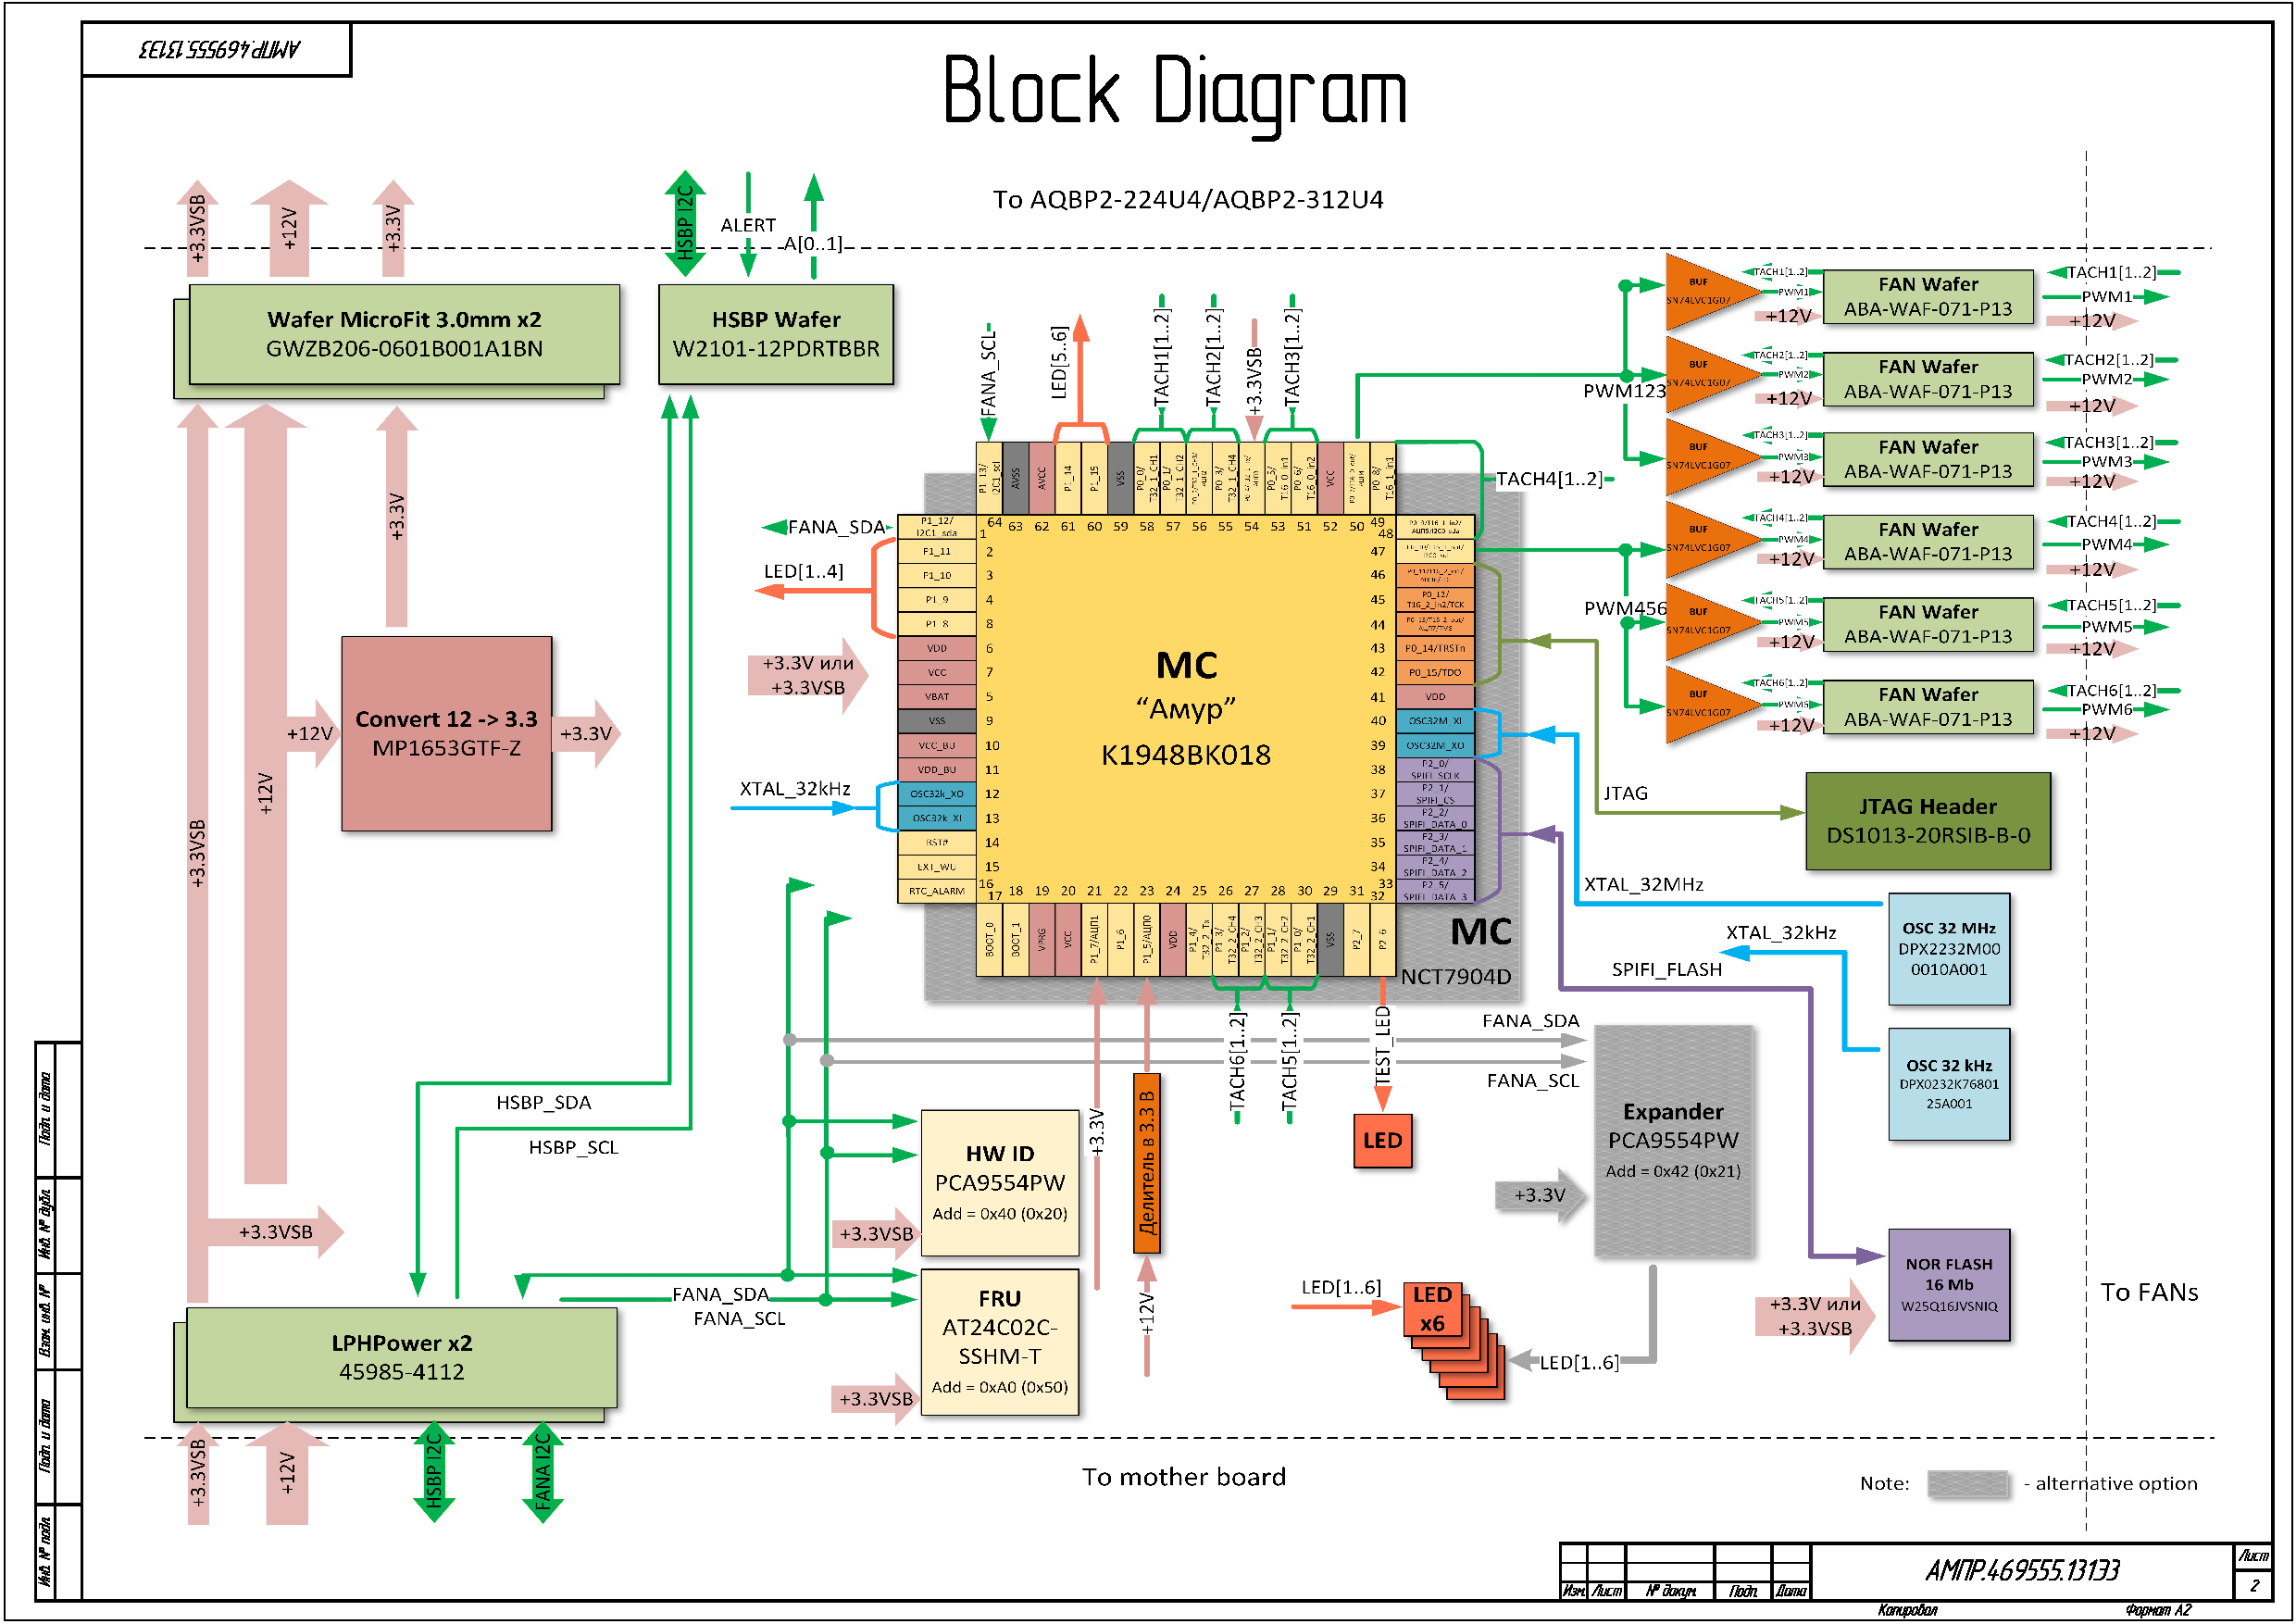
\includepdf[pages=-, pagecommand={}, angle=90, scale=0.70]{appendix-midplane.pdf}
\end{figure}

\chapter{Схема Heating Unit}

\begin{figure}[H]
	\centering
	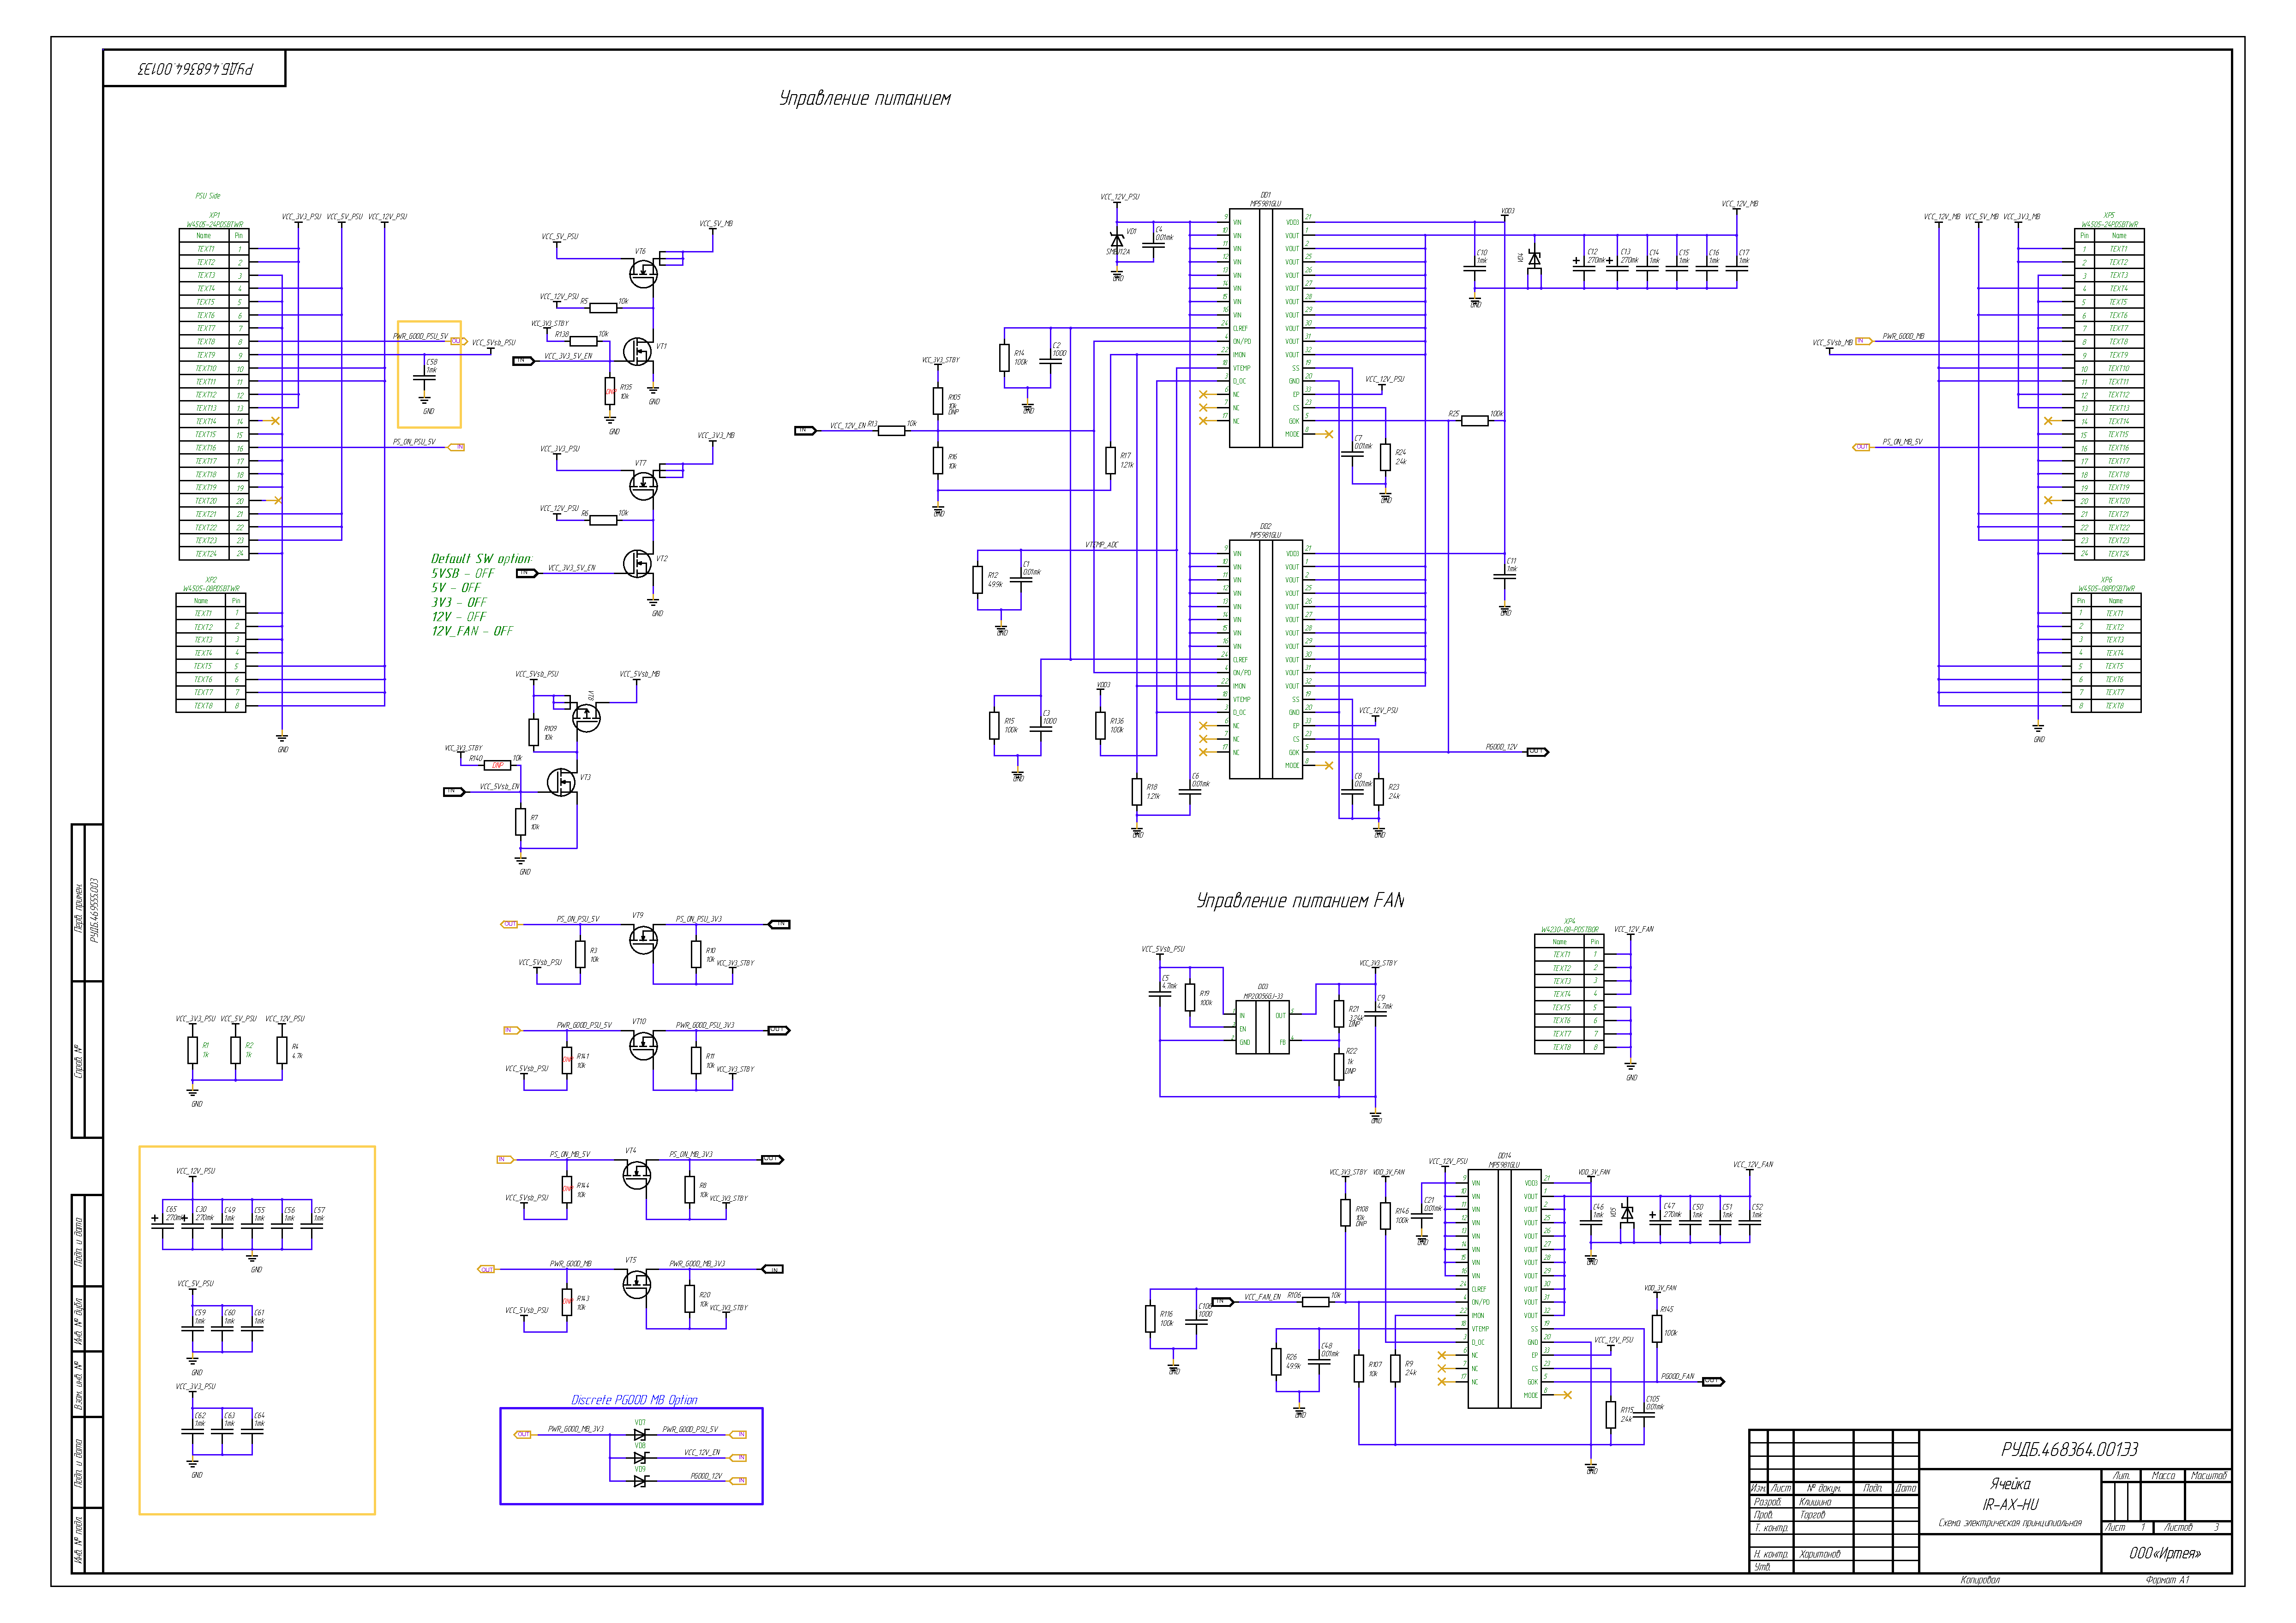
\includepdf[pages=1, pagecommand={}, angle=90, scale=0.75]{appendix-hu.pdf}
\end{figure}

\includepdf[pages=2, pagecommand={}, angle=90, scale=0.85]{appendix-hu.pdf}
\includepdf[pages=3, pagecommand={}, angle=90, scale=0.85]{appendix-hu.pdf}


\end{document}

%%% Local Variables:
%%% mode: latex
%%% TeX-master: t
%%% End:
